\thispagestyle{empty}


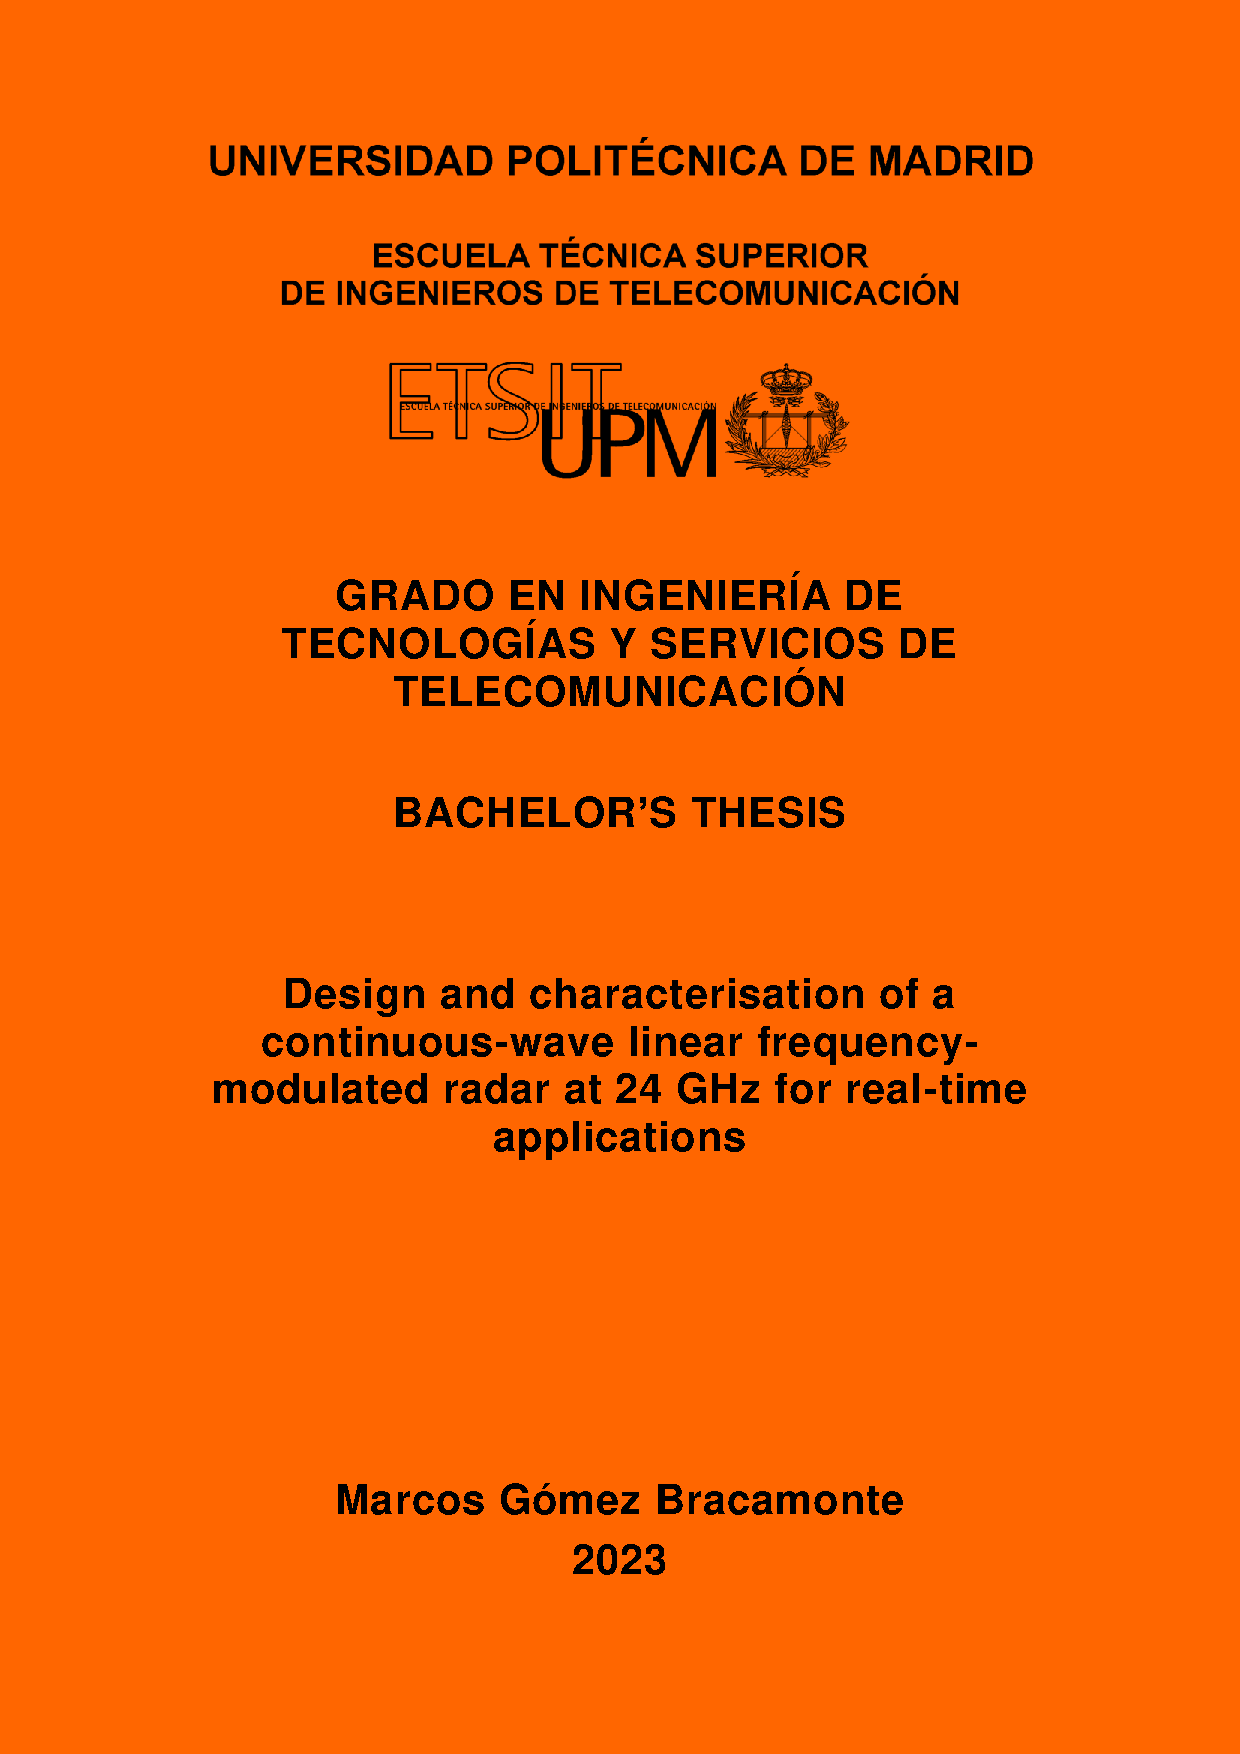
\includepdf{cover/PortadaMUIT.pdf}    


\pagebreak[1] \clearpage
%\thispagestyle{empty}%
\vspace*{-1cm}

\begin{hyphenrules}{nohyphenation}
	\textbf{GRADO EN INGENIERÍA DE TECNOLOGÍAS Y SERVICIOS DE TELECOMUNICACIÓN}\\[2cm]
\end{hyphenrules}
\textbf{TRABAJO FIN DE GRADO}\\
{\setlength{\extrarowheight}{20pt}%
\begin{tabular}{@{}lp{0.6\linewidth}@{}}
	\textbf{Título:} & \titulo \\
	\textbf{Autor:} & \autor  \\
	\textbf{Tutor:} & \director  \\
	\textbf{Ponente:} & \ponente \\
	\textbf{Departamento:} &  Señales, Sistemas y Radiocomunicaciones\\
\end{tabular}}

\vspace{1cm}
\textbf{MIEMBROS DEL TRIBUNAL}\\
{\setlength{\extrarowheight}{20pt}%
	\begin{tabular}{@{}lp{0.6\linewidth}@{}}
		\textbf{Presidente:} &  \\
		\textbf{Vocal:} &   \\
		\textbf{Secretario:} & \\
		\textbf{Suplente:} &   \\
\end{tabular}}

\vspace{1cm}
Los miembros del tribunal arriba nombrados acuerdan otorgar la calificación de:\\[1cm]

\begin{flushright}
	Madrid, a \hspace{2cm} de \hspace{4cm} de 20 \hspace{0.5cm}
\end{flushright}

\thispagestyle{empty}

\clearpage

\thispagestyle{empty}
\begin{titlepage}
\begin{center}
	\textsc{\Large UNIVERSIDAD POLITÉCNICA DE MADRID }\\
	
	\vspace{0.8cm}
	{\large ESCUELA TÉCNICA SUPERIOR\\DE INGENIEROS DE TELECOMUNICACIÓN} \\
\end{center}
\begin{center}
	
\includegraphics[width=6cm]{cover/anagrama}     %%%%%Escudito
\end{center}

\vspace{1.5cm}
\begin{center}
	{\Large GRADO EN INGENIERÍA DE TECNOLOGÍAS Y SERVICIOS DE TELECOMUNICACIÓN} \\
	\vspace{1cm}
	
	{\Large BACHELOR'S THESIS} \\
	
\end{center}


\begin{center}
	\vspace{1.5cm}
		{\LARGE \expandafter{\textbf{\titulo}}}
\end{center}

\vspace{3.5cm}
\begin{center}
	\textrm
	{\Large \autor}
\end{center}

\begin{center}
	\vspace{1.5cm}
	{\Large 2023}
\end{center}
\end{titlepage}
\pagebreak[1] \clearpage
\thispagestyle{empty}%



%\pagebreak[1] \thispagestyle{empty}
%%%%%%%%%%%%%%%%%%%%%%%%%% P�gina en blanco
%\pagebreak[1] \vfill \clearpage \thispagestyle{empty} \quad
%\clearpage
%%%%%%%%%%%%%%5
%%%%%%%%%%%%%%%%%%%%%%%%%% P�gina en blanco
%\pagebreak[1] \vfill \clearpage \thispagestyle{empty} \quad
%\clearpage
%%%%%%%%%%%%%%5
%%%%%%%%%%%%%%%%%%%%%%%%%% P�gina en blanco
%\pagebreak[1] \vfill \clearpage \thispagestyle{empty} \quad
%\clearpage
%%%%%%%%%%%%%%5
%\thispagestyle{empty}
%     \begin{center}
	%         \sc{\small DEPARTAMENTO DE SISTEMAS, SEÑALES Y RADIOCOMUNICACIONES\\}
	%          \vspace{0.5cm}
	%          Escuela Técnica Superior de Ingenieros de Telecomunicación\\
	%          Universidad Politécnica de Madrid
	%     \end{center}
%     \vspace{3cm}
%     \begin{center}
	%          {\Large\uppercase\expandafter{\titulo}}
	%     \end{center}

%     \vspace{0.5cm}
%     \begin{center}
	%          {\large TRABAJO FIN DE MASTER}
	%     \end{center}
%     \vspace{3cm}

%     \begin{center}
	%          \rm Autor:\\
	%          \par \vspace{0.2cm}
	%          {\Large  \autor}\\
	%          \par \vspace{0.1cm}
	%          \end{center}
%     \vspace{2cm}
%   \begin{center}
	%        \rm Tutor:\\
	%        \par \vspace{0.2cm}
	%        {\Large \director}\\
	%        \par \vspace{0.1cm}
	%        \directortitulo\\
	%   \end{center}

%\pagebreak[1] \clearpage
%\thispagestyle{empty}%
%\vspace*{-1cm}
%\noindent
%\textbf{TÍTULO}:\hspace{2.3cm} \parbox[t]{10cm}{\uppercase{\titulo}} %\vspace{.5cm} \\[2mm]
%\textbf{AUTOR}: \hspace{2.3cm} \autor\\[3mm]
%\textbf{TUTOR}: \hspace{2.3cm} \director\\[3mm]
%\textbf{DEPARTAMENTO}: \hspace{.05cm} Señales, Sistemas y %Radiocomunicaciones\\[3mm]
%\noindent
%\textbf{MIEMBROS DEL TRIBUNAL CALIFICADOR}\\[7mm]
%\noindent
%\hspace*{0.5cm} \textbf{PRESIDENTE}: \hspace{0.5cm} D. ALBERTO ASENSIO LÓPEZ\\[3mm]
%\noindent
%\hspace*{0.5cm} \textbf{VOCAL}: \hspace{1.9cm} D. MATEO BURGOS GARCÍA\\[3mm]
%\noindent
%\hspace*{0.5cm} \textbf{SECRETARIO}: \hspace{0.5cm} D. JESUS GRAJAL DE LA FUENTE\\[3mm]
%\noindent
%\hspace*{0.5cm} \textbf{SUPLENTE}: \hspace{1.05cm} D. JAVIER GISMERO MENOYO\\[7mm]
%\noindent
%\textbf{FECHA DE LECTURA}:\\[7mm]
%\noindent
%\textbf{CALIFICACIÓN}:\\[7mm]
%\noindent
%\vspace{0.2cm}
%%%%%%%%%%%%%%%%%%%%%%%%%% P�gina en blanco
%\pagebreak[1]  \thispagestyle{empty} 
%\clearpage
%%%%%%%%%%%%%%5
%nueva p�g. en blanco
%%%%%%%%%%%%%%%%%%%%%%%%%% P�gina en blanco
%\pagebreak[1] \vfill \clearpage \thispagestyle{empty} \quad
%\clearpage
%%%%%%%%%%%%%%5

\pagebreak[1] \clearpage
\thispagestyle{empty}%
\begin{center}
	(Page left blank)
\end{center}

\pagebreak[1] \vfill \clearpage \thispagestyle{empty} \quad
\thispagestyle{empty}
\begin{center}
	\textbf{\large ABSTRACT} \\
	\noindent\rule{10cm}{0.8pt}
\end{center}

In recent years, radar technology has been used for monitoring several diseases remotely and non-intrusively. This allows further comfort of the patient and enables better diagnostic results. Continuous-wave frequency-modulated radars are one of the most promising technologies. However, these radar systems usually do not provide real-time measurements, or if they do, the systems are very expensive. Moreover, most of the systems capable of performing real-time measurements lose information because they discard a large number of useful samples.
In this Bachelor Thesis, the design, development, measurement and characterisation of a continuous-wave frequency-modulated radar system operating in millimetre-band, specifically at 24 GHz, is carried out. The designed system is low-cost and provides a means to transmit the measured information in near real-time, guaranteeing signal integrity.
The radar is based on a commercially-available MMIC which outputs intermediate-frequency (IF) signals. The processing of these signals is performed by circuits designed in this Bachelor Thesis. These signals are conditioned and transmitted via Bluetooth Low Energy for real-time acquisition and processing. The figures of merit for the application are real-time, signal integrity and low-cost.
After manufacturing, the performance and operation of all parts of the radar system are analysed and measured using currently available laboratory equipment.
Finally, the radar is tested by measuring the gait of a person in the context of monitoring Parkinson's Disease.


\vspace{2cm}
\noindent \textbf{KEY WORDS:} CWFM radar, microdoppler, PD, gait analysis, real-time, Bluetooth Low Energy\\[3mm]


\pagebreak[1] \vfill \clearpage \thispagestyle{empty} \quad
\thispagestyle{empty}
%\pagebreak[1]
%\vfill \clearpage \thispagestyle{empty}
\thispagestyle{empty}
\begin{center}
	\textbf{\large RESUMEN} \\
	\noindent\rule{10cm}{0.8pt}
\end{center}

En los últimos años, la tecnología radar ha sido empleada para monitorizar varias enfermedades de manera remota y no invasiva. Así se proporciona un mayor confort al paciente y se consiguen mejores diagnósticos. Los radares de onda continua y frecuencia modulada son una de las tecnologías más prometedoras. No obstante, estos radares normalmente no proporcionan medidas en tiempo real, o si lo hacen, tienen un elevado coste. Además, muchos de los sistemas capaces de medir en tiempo real pierden información porque descartan gran cantidad de muestras útiles.
En este Trabajo de Fin de Grado se realiza el diseño, desarrollo, medición y caracterización de un radar de onda continua y frecuencia modulada en la banda de ondas milimétricas, específicamente a 24 GHz. El sistema diseñado es de bajo coste y es capaz de transmitir la información de las medidas en cuasi tiempo real, garantizando la integridad de la señal.
El radar se basa en un MMIC comercial, que genera señales de frecuencia intermedia (IF). El procesado de estas señales es llevado a cabo por unos circuitos de diseño propio. Estas señales se acondicionan y transmiten vía Bluetooth Low Energy para adquisición y procesado en tiempo real. Las figuras de mérito para esta aplicación son tiempo real, integridad de la señal y bajo coste.
Después de su fabricación, se analiza y mide el rendimiento y funcionamiento de todas las partes del radar con los equipos disponibles en el laboratorio.
Finalmente, el radar se prueba midiendo la marcha de una persona en el contexto de la monitorización de la Enfermedad de Parkinson.


\vspace{2cm}
\noindent \textbf{PALABRAS CLAVE:} radar CWFM, microdoppler, EP, análisis de la marcha, tiempo real, Bluetooth Low Energy\\[3mm]


\clearpage
